\KSe\ is one of the most studied models of 
complex \spt\ dynamics in spatially extended systems.
It was formulated
independently by Kuramoto in the context of angular phase
turbulence in reaction-diffusion systems\rf{KurTsu75}, and
by Sivashinsky in the study of hydrodynamic instability of laminar
flames\rf{michsiv77}. 
It also describes the instabilities of 
dissipative trapped ion modes in plasmas\rf{laquey74} and the 
flow of a viscous liquid film down a vertical wall\rf{ShSi82}.
Its one\dmn\ form is frequently written as 
\begin{equation}
  u_t+\frac{1}{2}(u^2)_x+u_{xx}+u_{xxxx}=0\,,\; x\in [0,L]
  \label{eq:ks}
\end{equation}
defined on a periodic domain $u(x, t) = u(x+L, t)$.
In the combustion formulation, $u(x, t)$ represents the 
flame front velocity. Everyday experience tells us that a candle flame
flickers and its shape changes quite often, without any exterior influence. 
Therefore, \KSe\ is expected to exhibit chaotic behaviors. 
\refFig{fig:KS_L100200} displays its \spt\ profiles with 
domain size $L=100$ and $200$ respectively. Recurrent patterns appear not 
only along the temporal axis but also along the spatial axis. This \spt\ 
chaotic behavior is also observed in other spatially-extended dynamical 
systems such as \cGLe\rf{SPScgl92}.
At the same time, \reffig{fig:KS_L100200} provides coarse information about
the time and length scale of this ``dimensionless'' system. 
In all our simulations, we set $L = 22$, which is large enough to exhibit
complex \spt\ chaotic dynamics{\rf{SCD07}}.

\begin{figure}
  \centering
  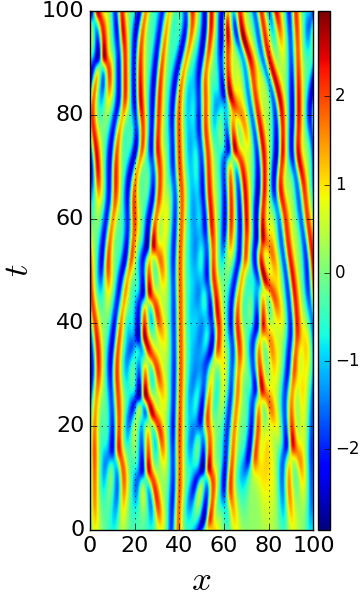
\includegraphics[height=0.35\textheight]{KS_L100N256}
  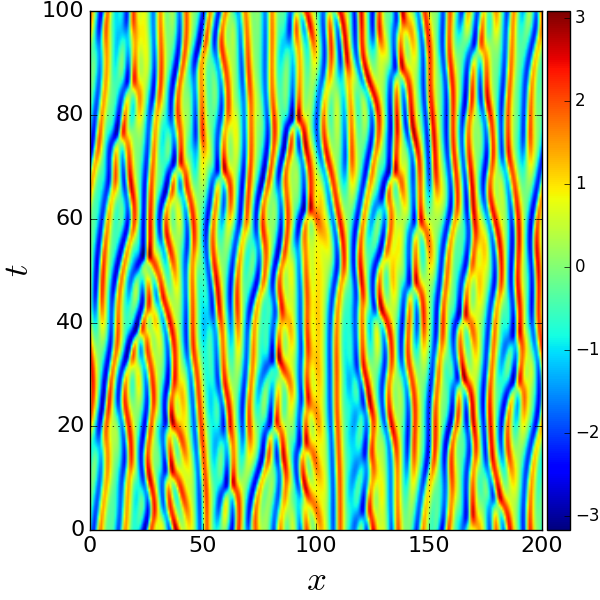
\includegraphics[height=0.35\textheight]{KS_L200N256}
  \caption[\Spt\ plots of the one\dmn\ \KSe\ for $L=100$ and $200$.]{
    Simulations of the one\dmn\ \KSe\ for domain size $L=100, 200$ respectively with random initial
    conditions. The color represents the magnitude of $u(x, t)$.
  }
  \label{fig:KS_L100200}
\end{figure}


\section{Numerical setup}
\label{sect:ksnumer}

Periodic boundary condition enables us to transform \refeq{eq:ks}
into a set of ODEs in the Fourier space
\begin{equation}
\dot{a}_k \;\; =
( q_k^2 - q_k^4 )\, a_k
- i \frac{q_k}{2} \sum_{m=-\infty}^{\infty}a_m a_{k-m}
\label{eq:ksfourier}
\end{equation}
where $q_k = 2\pi k/L$ and the coefficients are complex,
\[
  a_{k}=b_{k}+ic_{k}\,.
\] 
Pseudo-spectral method\rf{trefethenSpectral} 
is deployed to evaluate terms in \refeq{eq:ksfourier}. That is, the linear term is 
calculated in the Fourier space; while the nonlinear term is first transformed 
to the physical space, calculated there and then transformed back to the Fourier space.
In our simulations, discrete Fourier transform
is used with $N=64$ modes, \ie, $k = -N/2 + 1$ up to $N/2$ in \eqref{eq:ksfourier}.

Since $u(x,t)$ is real, $a_{k}(t)=a^{*}_{-k}(t)$; thus, only half of the
Fourier modes are independent. As $\dot{a}_{0}=0$ from
\eqref{eq:ksfourier}, we can set $a_{0}=0$ corresponding to
zero mean velocity without loss of generality.
Also, the nonlinear term
of $\dot{a}_{N/2}$, in fact, has coefficient
$-i(q_{N/2} + q_{-N/2})/2 = 0$
from symmetric consideration\rf{trefethenSpectral};
thus, $a_{N/2}$ is decoupled from other modes and it
can be set to zero as well. Therefore, the number of independent variables
is $N-2$,
\begin{equation}
  \label{eq:fourierspace}
  \cssp=(b_{1},c_{1},b_{2},c_{2},\cdots,b_{N/2-1},c_{N/2-1})^\top
  \,.
\end{equation}
This is the full \statesp\ in the discussion that follows. 

The stiffness caused by the quaternary term in the linear part
 makes popular integration methods such as
fourth order Runge-Kutta inefficient in this case. Therefore,
we resort to exponential integrators\rf{HoOs10, Montanelli2016} to
integrate the linear part exactly. In our simulations,
exponential time-differencing
scheme combined with fourth order Runge-Kutta\rf{cox02jcomp, ks05com}
is implemented to integrate
\eqref{eq:ksfourier}. By this scheme, 
a relatively large time step can be used to 
achieve a fourth-order global accuracy. 

